\section{LES of a Turbulent Premixed Methane Flame}
\subsection{Model Problem}


\begin{figure}
    \vspace{0.2cm}
    \begin{center}
      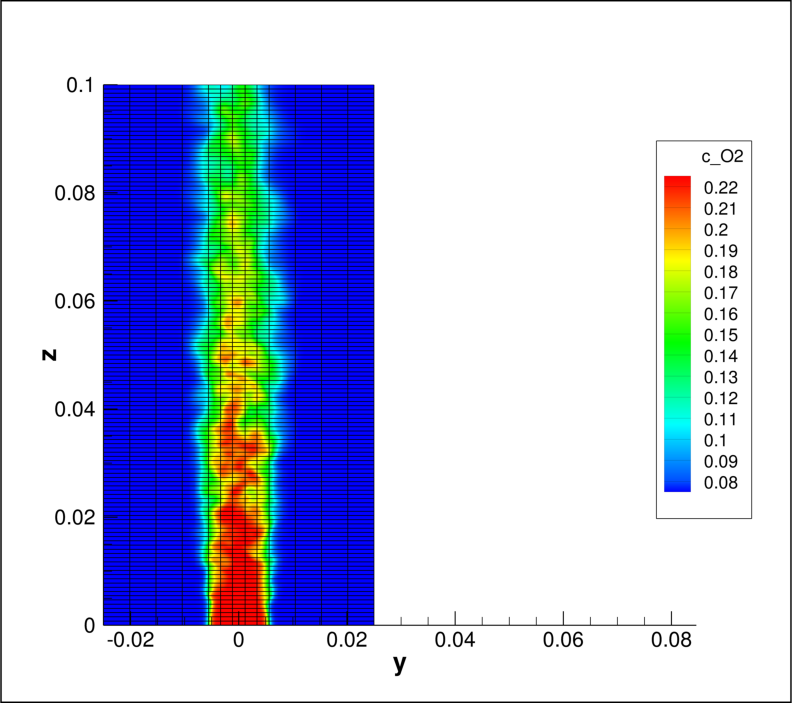
\includegraphics[height=0.4\textwidth]{./figs/Time_averaged_c_O2.png}
    \end{center}
    \caption{Time averaged $O_2$ species concentration}  
    \vspace{0.2cm}
    \label{fig:oxygen}	
\end{figure}

The CFFC code was used to run a simulation for a Turbulent Premixed Methane flame, using 800 nodes, 3200 blocks and each block having $8^3 = 512$ cells, hence a total of $1,638,400$ cells. Time averaged results for t=6ms, 7ms, 8ms, 9ms, 10ms and 11ms are shown in figure \ref{fig:oxygen}, the contours representing the species concentration of Oxygen.\par


Included here are some pictures from previous CFFC simulations that show the varying mesh cell sizes among the different blocks.

\begin{figure}[t!]
  \centering
   \subfigure[At t=2.0ms, 800 (8x8x8) blocks, ~410,000 cells
(no refinement, 1 mesh level)]
   {\label{fig:2msflame}	   
   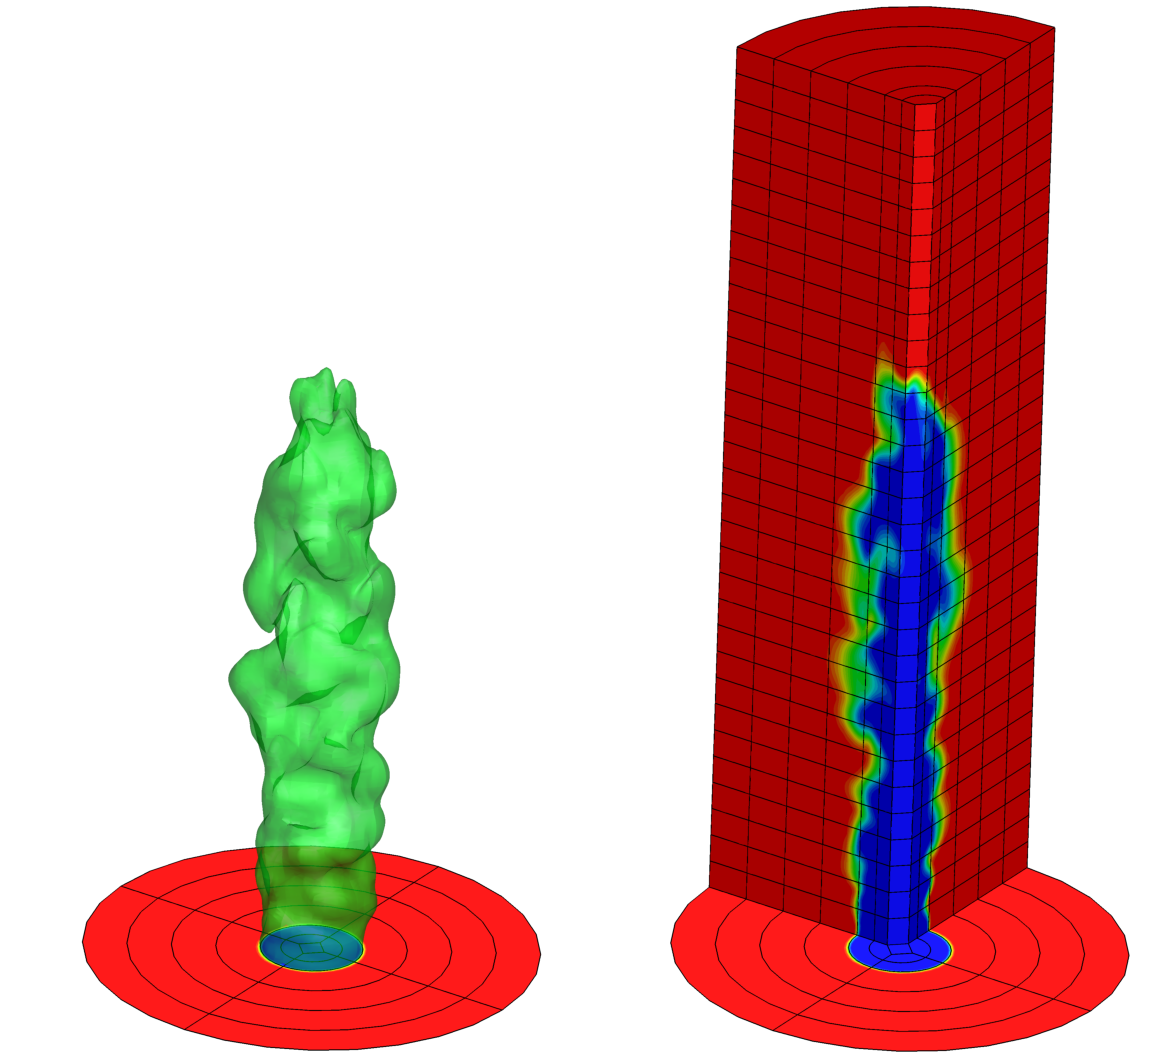
\includegraphics[height=0.25\textwidth]{figs/fsd2_0ms.png}}%
	\:
	\subfigure[At t=4.25ms 5595 (8x8x8) blocks, ~2.8 million cells
(3 levels of mesh refinement)]
   {\label{fig:4msflame}	   
   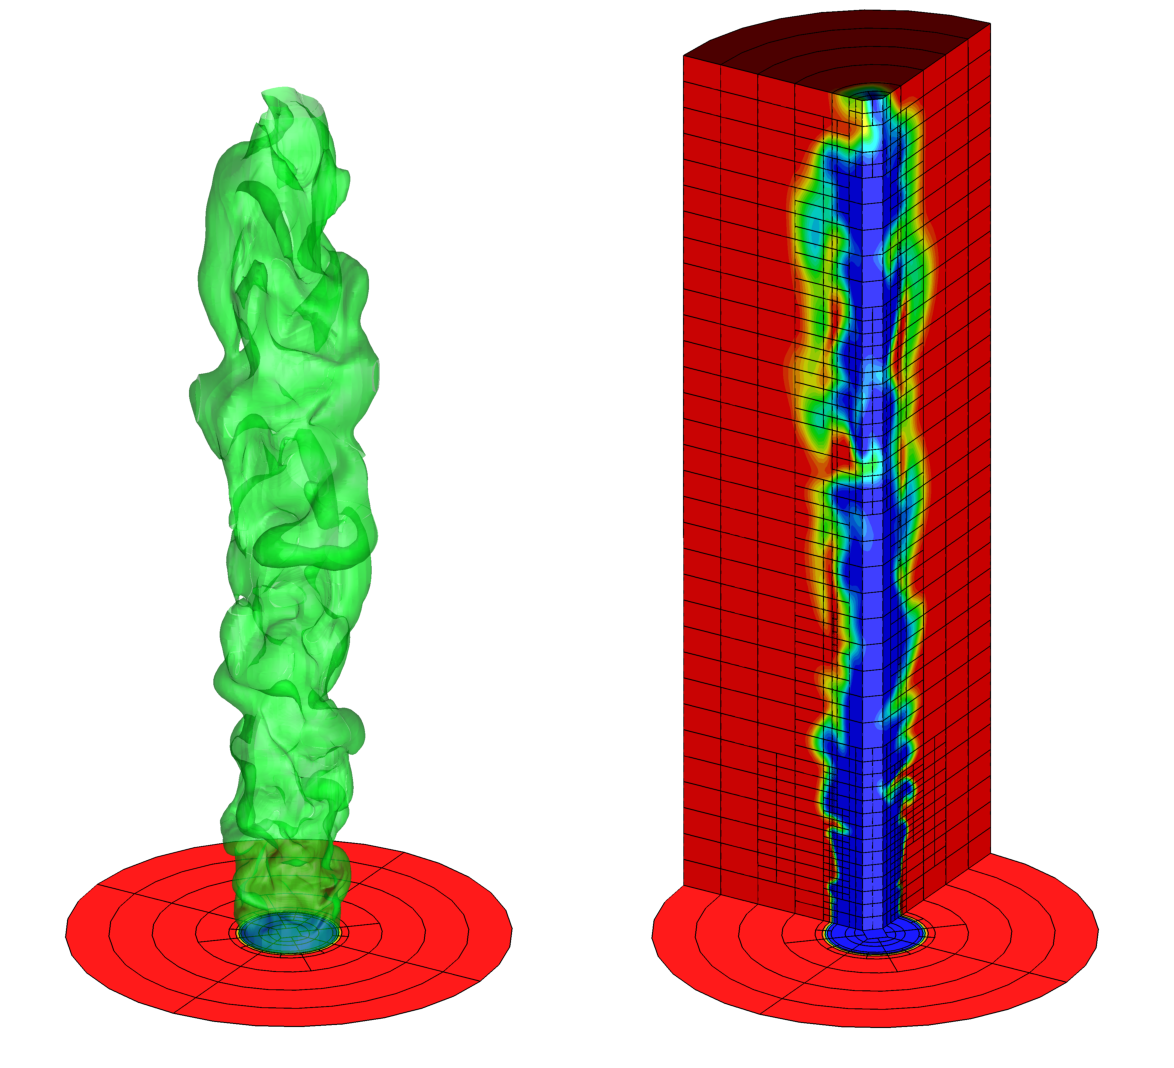
\includegraphics[height=0.25\textwidth]{figs/fsd4_25ms.png}}%
   \:
	\subfigure[At 7.0 ms, 18531 (8x8x8) blocks, ~9.5 million cells
(3 levels of mesh refinement)]
   {\label{fig:7msflame}	   
   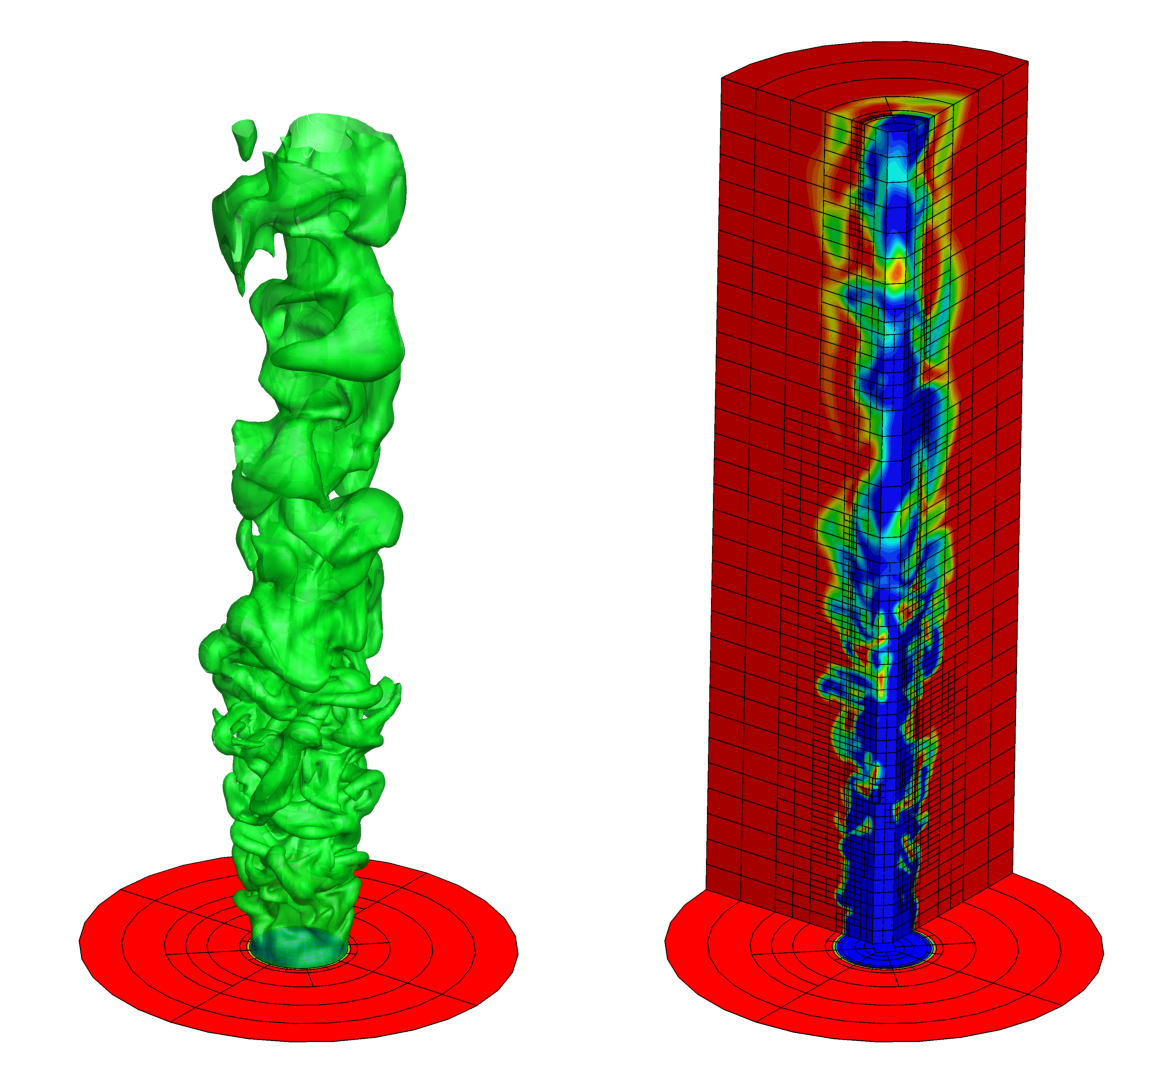
\includegraphics[height=0.25\textwidth]{figs/fsd7_0ms.png}}%
   \caption{Some figures showing isotropic mesh refinement with 3 levels of refinement for a lean premixed methane air flame in air. LES solutions were obtained with the flame surface density (FSD) model and the refinement was based on temperature gradient.} 
      
\end{figure}  


